\section{Results}
\label{sec:results}


\begin{figure}[H]
  \centering
  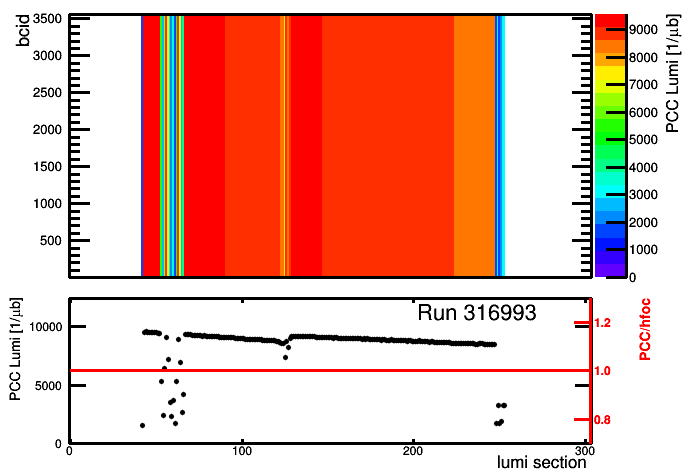
\includegraphics[width=0.5\columnwidth]{./316993.png}
  \caption{Top: Bunch crossing id (bcid) and PCC lumi as a function of lumi section. Bottom: PCC lumi as a function of lumi section (late RunD veto list is used) for run 2018A.}
  \label{fig:CMS}
\end{figure}


\begin{figure}[H]
  \centering
  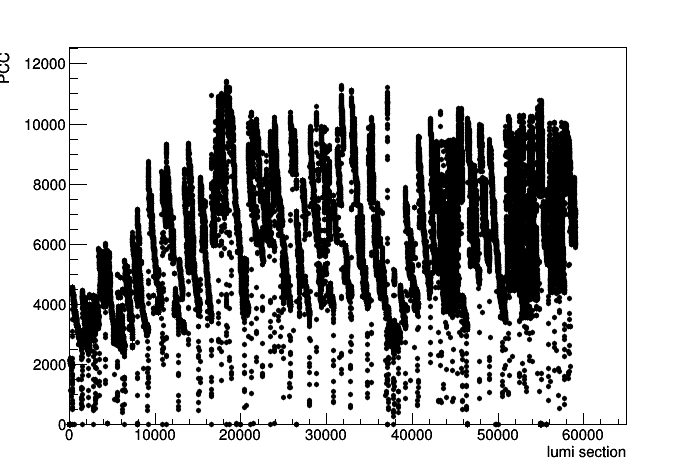
\includegraphics[width=0.5\columnwidth]{./ls_lumi.png}
  \caption{PCC luminosity as a function of lumi section.}
  \label{fig:CMS}
\end{figure}


\begin{figure}[H]
  \centering
  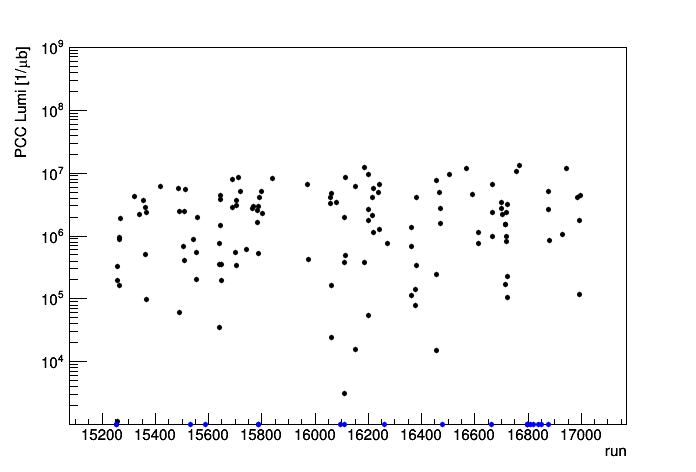
\includegraphics[width=0.5\columnwidth]{./runs.png}
  \caption{PCC luminosity as a function of run number.}
  \label{fig:CMS}
\end{figure}


\begin{figure}[H]
  \centering
  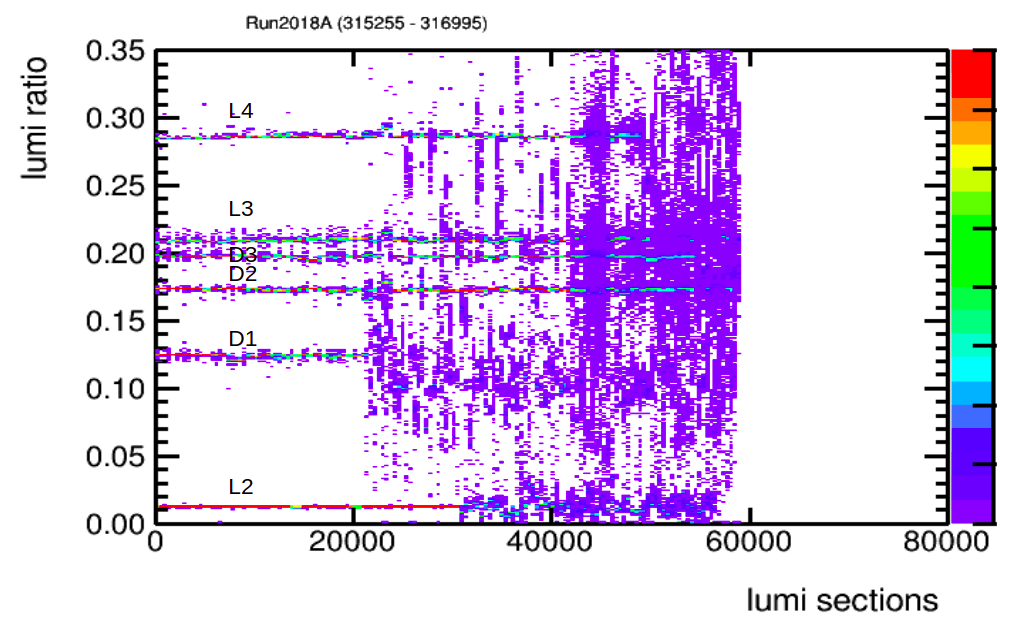
\includegraphics[width=0.5\columnwidth]{./2018A_lumiratio.png}
  \caption{Luminosity ratios for different subdetectors L2, L3, L4, D1, D2, D3 of pixel detector as a function of lumi section for Run2018A.}
  \label{fig:CMS}
\end{figure}



\begin{figure}[H]
  \centering
  \includegraphics[width=0.5\columnwidth]{./ProfileXcombined_2018A.png}
  \caption{X Profile of luminosity ratio vs lumi section graph showing luminosity fraction as a function of lumi section.}
  \label{fig:CMS}
\end{figure}





\begin{figure}[H]
  \centering
  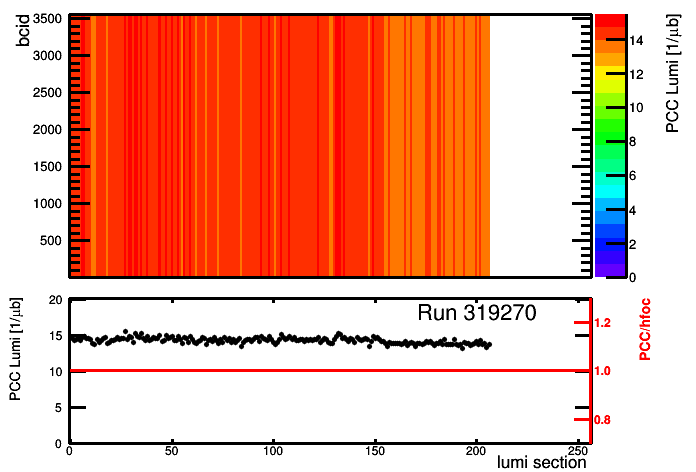
\includegraphics[width=0.5\columnwidth]{./319270.png}
  \caption{Top: Bunch crossing id (bcid) and PCC lumi as a function of lumi section. Bottom: PCC lumi as a function of lumi section (late RunD veto list is used) for run 2018B.}
  \label{fig:CMS}
\end{figure}


\begin{figure}[H]
  \centering
  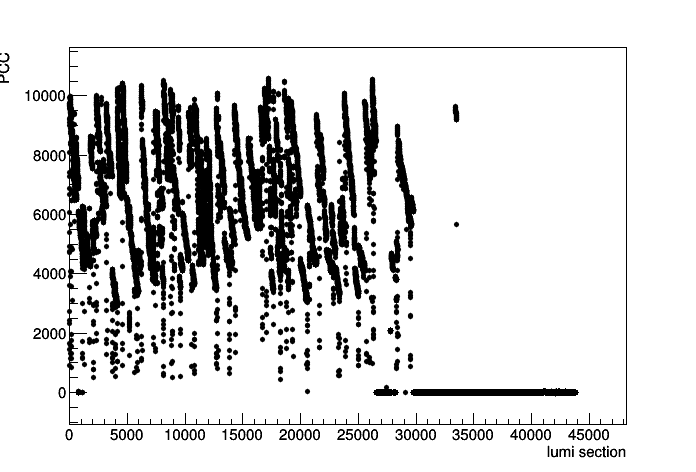
\includegraphics[width=0.5\columnwidth]{./ls_lumi_2018B.png}
  \caption{PCC luminosity as a function of lumi section.}
  \label{fig:CMS}
\end{figure}


\begin{figure}[H]
  \centering
  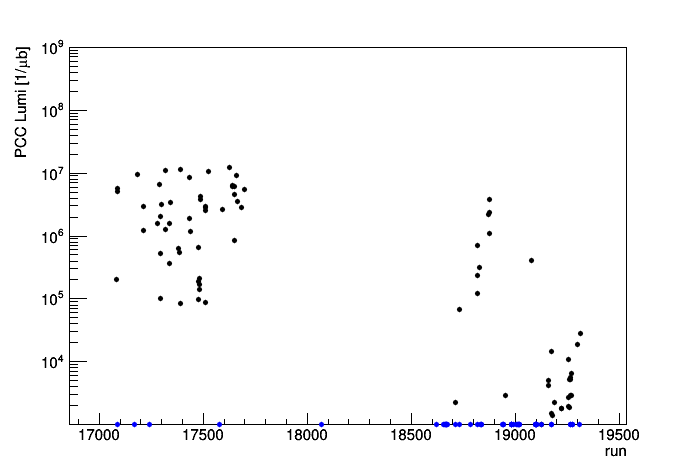
\includegraphics[width=0.5\columnwidth]{./runs_2018B.png}
  \caption{PCC luminosity as a function of run number.}
  \label{fig:CMS}
\end{figure}


\begin{figure}[H]
  \centering
  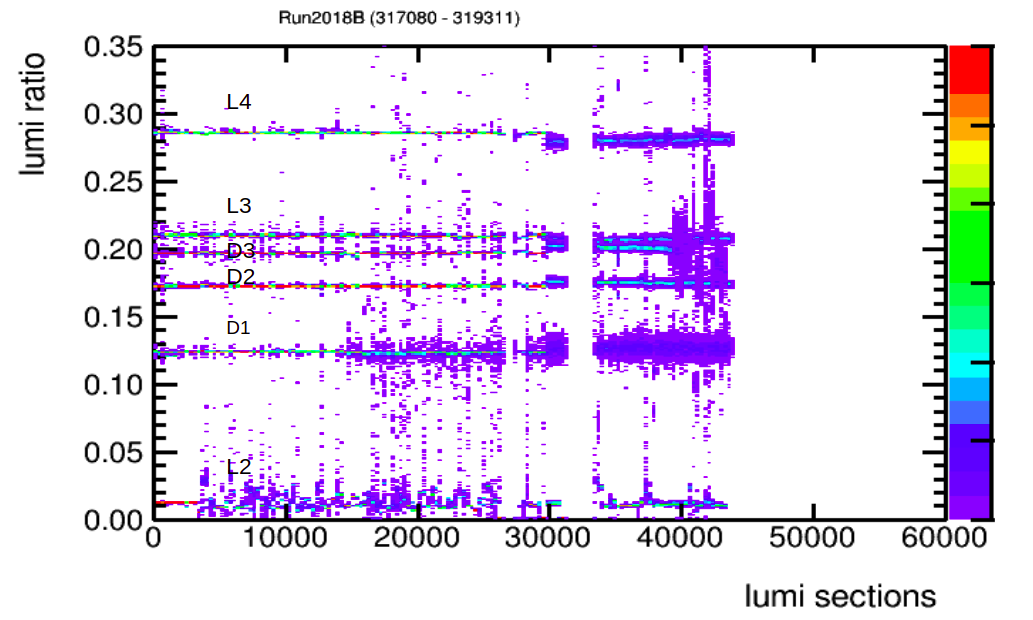
\includegraphics[width=0.5\columnwidth]{./2018B_lumiratio.png}
  \caption{Luminosity ratios for different subdetectors L2, L3, L4, D1, D2, D3 of pixel detector as a function of lumi section for Run2018B.}
  \label{fig:CMS}
\end{figure}



\begin{figure}[H]
  \centering
  \includegraphics[width=0.5\columnwidth]{./ProfileXcombined_2018B.png}
  \caption{X Profile of luminosity ratio vs lumi section graph showing luminosity fraction as a function of lumi section.}
  \label{fig:CMS}
\end{figure}



\begin{figure}[H]
  \centering
  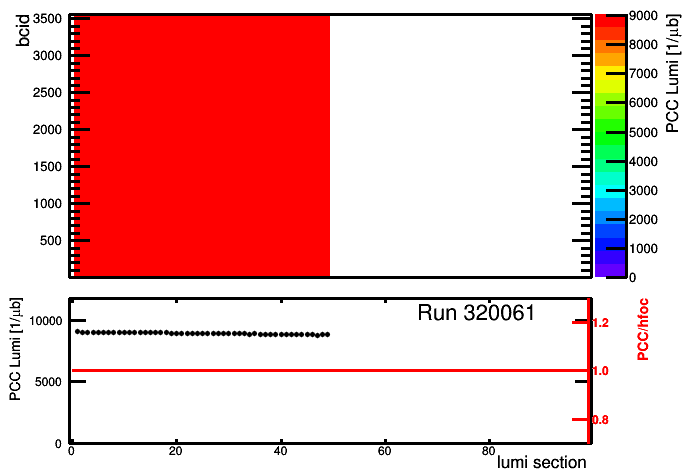
\includegraphics[width=0.5\columnwidth]{./320061.png}
  \caption{Top: Bunch crossing id (bcid) and PCC lumi as a function of lumi section. Bottom: PCC lumi as a function of lumi section (late RunD veto list is used) for run 2018C.}
  \label{fig:CMS}
\end{figure}


\begin{figure}[H]
  \centering
  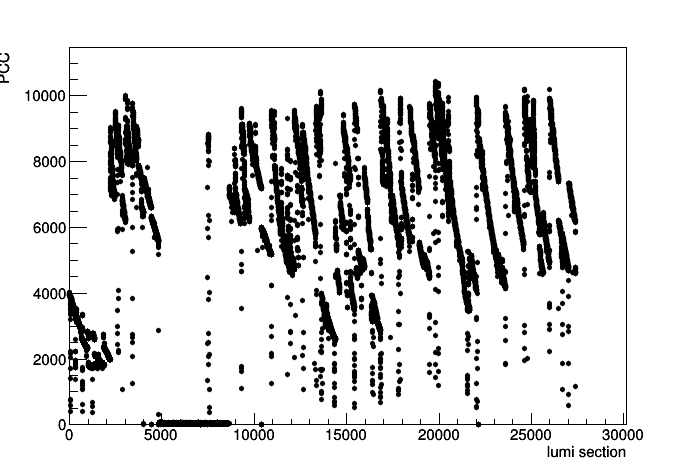
\includegraphics[width=0.5\columnwidth]{./ls_lumi_2018C.png}
  \caption{PCC luminosity as a function of lumi section.}
  \label{fig:CMS}
\end{figure}


\begin{figure}[H]
  \centering
  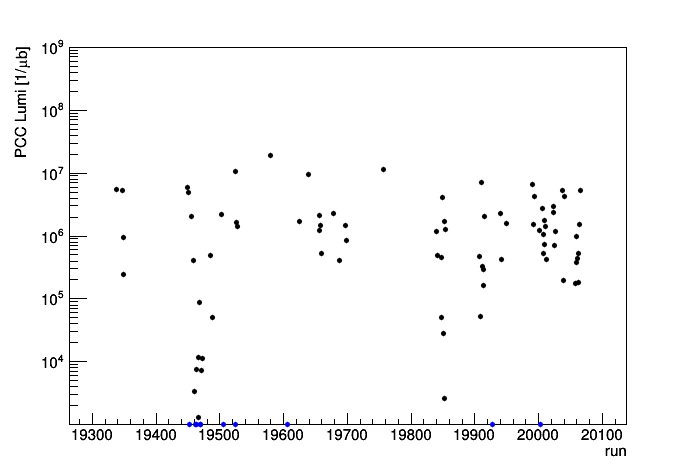
\includegraphics[width=0.5\columnwidth]{./runs_2018C.png}
  \caption{PCC luminosity as a function of run number.}
  \label{fig:CMS}
\end{figure}


\begin{figure}[H]
  \centering
  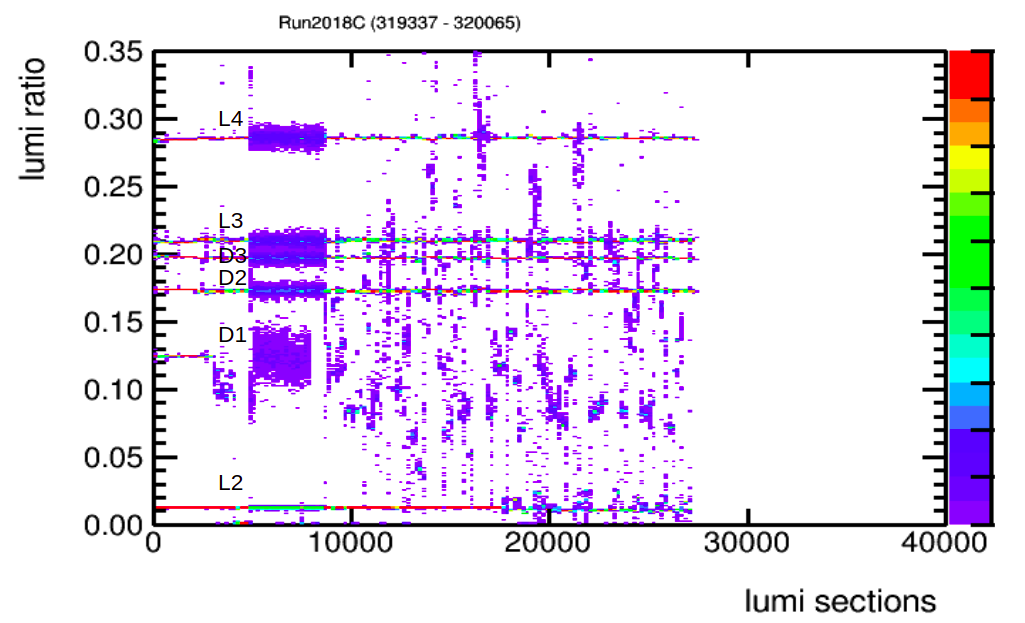
\includegraphics[width=0.5\columnwidth]{./2018C_lumiratio.png}
  \caption{Luminosity ratios for different subdetectors L2, L3, L4, D1, D2, D3 of pixel detector as a function of lumi section for Run2018C. }
  \label{fig:CMS}
\end{figure}


\begin{figure}[H]
  \centering
  \includegraphics[width=0.5\columnwidth]{./ProfileXcombined_2018C.png}
  \caption{X Profile of luminosity ratio vs lumi section graph showing luminosity fraction as a function of lumi section.}
  \label{fig:CMS}
\end{figure}
